%
% 2_Multipol.tex
%
% (c) 2020 Prof Dr Andreas Müller, Hochschule Rapperswil
%
% !TEX root = ../../buch.tex
% !TEX encoding = UTF-8
%
\section{Multipolmoment
\label{planet:section:multipol}}
\rhead{Multipolmoment}
In der Physik ist die Multipolentwicklung ein Verfahren, um die Poisson-Gleichung im dreidimensionalen Raum zu lösen, wobei eine Laurent-Reihe als Lösungsfunktion entsteht.
Die Entwicklungskoeffizienten dieser Reihe heissen Multipolmomente.
Diese Methode wird hauptsächlich in der Elektrostatik und Magnetostatik verwendet, kann aber auf jedem Gebiet der Physik verallgemeinert werden, in dem die Poisson-Gleichung auftritt.

Die Motivation der Multipolentwicklung liegt darin, das Verhalten von beliebigen Potentialen (Gravitationspotential) in grosser Entfernung zu betrachten.
Analog zur Fourier-Theorie lässt sich mit der Multipolentwicklung ein komplexes physikalisches Problem in kleinere Teilprobleme aufteilen, die leichter zu lösen sind.
Die \cref{planet:fig:multipol} zeigt die ersten drei Entwicklungsschritte einer Ladungswolke.
Desweiteren zeigt sich auch, dass die Bewegungsgleichung für Planeten im wesentlichen zu linearen Differentialgleichungen für die Multipolkoeffizienten werden.
Alle Koeffizienten konvergieren gegen 0, ausser dem konstanten Koeffizienten, dieser ergibt die Kugelform.

Dieser Abschnitt und die Herleitungen basieren auf \cite{planet:multi} und \cite{planet:quadro}.

\begin{figure}[h!]
    \centering
    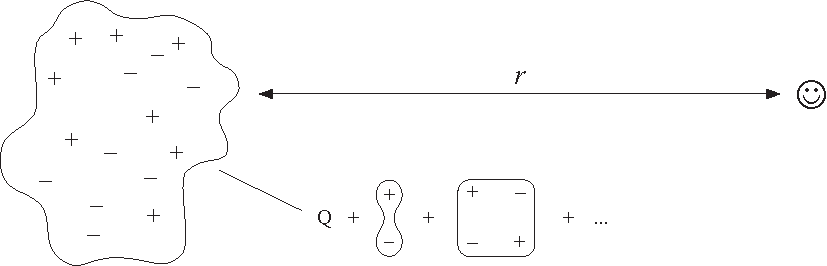
\includegraphics[width=\linewidth]{papers/planet/pictures/Multipol.pdf}
    \caption{Darstellung der Multipolentwicklung
        \label{planet:fig:multipol}}
\end{figure}

\subsection{Grundlagen
\label{planet:subsection:grundlagen}}

Die Poisson-Gleichung lässt sich allgemein als

\begin{equation*}
\Delta \phi (\vec{r}) = - f (\vec{r})
\end{equation*}

\noindent
schreiben, wobei \(\Delta\) der Laplace-Operator, \(f\) eine Dichte und \(\phi\) ein Potential ist (das Minus ist Konvention).
Die formale Lösung dieser Gleichung ist

\begin{equation*}
\phi (\vec{r}) = \frac{1}{4\pi} \int d^3 \vec{r}\,' \frac{f (\vec{r}\,')} {\abs{\vec{r} - \vec{r}\,'}}.
\end{equation*}

\noindent
Ist \(f (\vec{r})\) in einem Volumen lokalisiert, kann für Orte \(\vec{r}\), die weit ausserhalb dieses Volumens liegen, \(r \gg r\,'\), der Bruch in eine Taylor-Reihe in \(\vec{r}\,'\) um \(\vec{r}\,' = 0\) entwickelt werden:

\begin{equation*}
\frac{1}{\abs{\vec{r} - \vec{r}\,'}} = \sum_{n=0}^{\infty} \frac{1}{n!} \left( \vec{r}\,' \cdot \vec{\nabla}\,' \right)^n \left. \frac{1}{\abs{\vec{r} - \vec{r}\,'}} \right|_{\vec{r}\,'=0}
\end{equation*}

\noindent
Dabei bedeutet \(\vec{\nabla}\,'\), dass der Nablaoperator \(\vec{\nabla}\) nur auf die gestrichenen Koordinaten \(\vec{r}\,'\) und nicht auf \(\vec{r}\) wirkt.
Nach Bilden der Ableitungen werden diese an der Stelle \(\vec{r}\,' = 0\) ausgewertet.
Durch Umformen erhält man

\begin{equation*}
\frac{1}{\abs{ \vec{r} - \vec{r}\,'}} = \sum_{n=0}^{\infty} \frac{1}{n!} \left( - \vec{r}\,' \cdot \vec{\nabla} \right)^n \frac{1}{r}.
\end{equation*}

\noindent
Die genaue Form der Entwicklung und der Multipole hängt vom jeweiligen Koordinatensystem ab.

\subsection{Kartesische Multipolentwicklung
\label{planet:subsection:kartentwicklung}}

Die kartesische Multipolentwicklung wird im kartesischen Koordinatensystem durchgeführt.
Dort ist

\begin{equation*}
\vec{r}\,' \cdot \vec{\nabla} = r\,'_{i} \partial_{i},
\end{equation*}

\noindent
wobei die einsteinsche Summenkonvention verwendet wird.
Dann muss bei einem Summanden \(n\)-ter Ordnung ein Tensor \(n\)-ter Stufe, nämlich \(\textstyle \prod_{k=1}^{n} \partial_{i_{k}} \frac{1}{r}\) berechnet werden:


\begin{align*}
\frac{1}{\abs{ \vec{r} - \vec{r}\,'}} &= \frac{1}{r} - r\,'_{i} \partial_{i} \frac{1}{r} + \frac{1}{2} r\,'_{i} r\,'_{j} \partial_{i} \partial_{j} \frac{1}{r} + \mathcal{O}(r\,'^{3}) \\
&= \frac{1}{r} + r\,'_{i} \frac{r_{i}}{r^{3}} + \frac{1}{2} r\,'_{i} r\,'_{j} \frac{3 r_{i} r_{j} - r^{2} \delta_{i\!j}}{r^{5}} + \mathcal{O}(r\,'^{3}).
\end{align*}


\noindent
Das Symbol \(\delta_{i\!j}\) repräsentiert das sogenannte Kronecker-Delta.
Die formale Lösung \(\phi (\vec{r})\) der Poisson-Gleichung ist unter Verwendung der Identität \(r\,'_{i} r\,'_{j} r^{2} \delta_{i\!j} = r\,'^{2} r_{i} r_{j} \delta_{i\!j}\) wie folgt darstellbar:


\begin{align*}
\phi (\vec{r}) &= \frac{1}{4\pi} \Biggl[ \frac{1}{r} \underbrace{\int f (\vec{r}\,') \, d^3 \vec{r}\,'}_{\text{Monopol-}} + \frac{r_{i}}{r^{3}} \underbrace{\int d^3 \vec{r}\,' \, r\,'_{i} f (\vec{r}\,')}_{\text{Dipol-}} + \frac{1}{2} \frac{r_{i} r_{j}}{r^{5}} \underbrace{\int d^3 \vec{r}\,' \left( 3 r\,'_{i} r\,'_{j} - r\,'^{2} \delta_{i\!j} \right) f (\vec{r}\,')}_{\text{Quadrupolmoment}} \ldots \Biggr] \\
&= \frac{1}{4\pi} \left[ \frac{1}{r} q + \frac{r_{i}}{r^{3}} p_{i} + \frac{1}{2} \frac{r_{i} r_{j}}{r^{5}} Q_{i\!j} + \ldots \right].
\end{align*}


In der entwickelten Reihe kommen die Faktoren \(r\) im Nenner mit steigendem Exponenten vor.
Dabei werden die höheren Ordnungen der Multipolmomente, mit zunehmendem Abstand zum beobachteten Volumen immer weiter vernachlässigbar.
Der Einfachheit halber wurde für die Berechnungen der Kugelform in diesem Kapitel das erste Moment als Approximation verwendet und die höheren Momente vernachlässigt.



\subsection{Anwendung
\label{planet:subsection:anwendung}}

Die Gravitation hat im Gegensatz zum Elektromagnetismus nur positive Ladungen, die Massen.
Es können dennoch gravitative Multipole definiert werden.
Aus der Poisson-Gleichung des Newtonschen Gravitationsgesetzes

\begin{equation*}
    \Delta \phi = -4\pi G\rho
\end{equation*}

\noindent
mit der Gravitationskonstante \(G\) und der Massendichte \(\rho\) ist der gravitative Monopol die Gesamtmasse \(M\).

Da Massen nur positiv sind, lässt sich aus den Ladungen kein Dipolmoment bilden.
Aus diesem Grund ist der gravitative Quadrupol nicht über zwei Dipole definiert.
Dennoch haben Massenverteilungen Quadrupole.
\cref{planet:fig:quadroearth} zeigt ein solches wobei, die blau gefärbten Abweichungen, das Fehlen der Masse, als negative Masse gesehen wird und die rot gefärbten Abweichungen, die überschüssige Masse als positive Masse betrachtet wird.  

\begin{figure}[h]
    \centering
    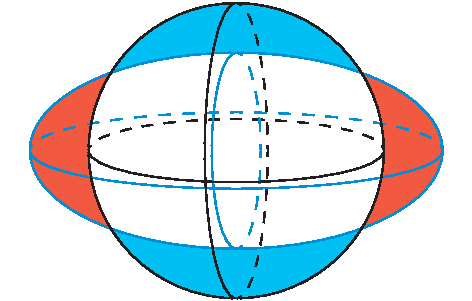
\includegraphics[width=0.60\linewidth]{papers/planet/pictures/Quadroearth.pdf}
    \caption{Beispiel eines gravitativen Quadrupols
        \label{planet:fig:quadroearth}}
\end{figure}

\begin{beispiel}
    Die Erde ist durch ihre Rotation keine perfekte Kugel, sie ist an den Polen leicht eingedellt und am Äquator bildet sich ein Wulst (\cref{planet:fig:quadroearth}).
    Die Schwerkraft versucht den höhren Multipolen entgegenzuwirken.
    Ausserdem ergeben sich durch bestimmte Dichteunterschiede weitere Abweichungen der Kugelform, in \cref{planet:fig:geoid} ersichtlich.
\end{beispiel}

Einige himmelsmechanische Phänomene, wie die dynamische Entwicklung der Bahnelemente von Satelliten, lassen sich mit dem daraus resultierenden Quadrupolmoment beschreiben.
